\chapter{Derivations}
\label{chap:derivations}

\section{Problem Statement and Challenges}
\label{sec:problemstatement}
The goal of this thesis is to perform a physically accurate and interactive simulation of structural color production as shown in figure $\ref{fig:problemstatementoutput}$, which we can see whenever light is diffracted from a natural grating. For this purpose we need the following input data (see figure $\ref{fig:problemstatement}$):
\begin{itemize}
  \item A mesh representing a snake surface$\footnote{In our simulation it is an actual reconstruction of a real snake skin. These measurements are provided by the Laboratory of Artificial and Natural Evolution at Geneva. See their website:\texttt{www.lanevol.org}.}$ as shown in figure $\ref{fig:strucgeom}$.
  \item A natural diffraction grating represented as a height field, its maximum height and its pixel width$\footnote{Since the nanostructure is stored as a grayscale image, we need a scale telling us what length and height one pixel corresponds to in this provided image.}$.
  \item A vector field which describes how the given nanostructure patch is oriented on the surface (see figure $\ref{fig:patchvectorfield}$). 
\end{itemize}

\begin{figure}[H]
  \centering
  \subfigure[Structure Geometry]{
    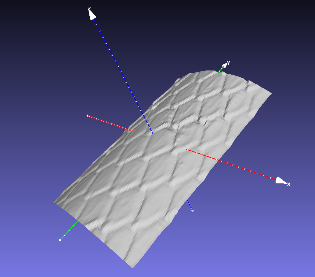
\includegraphics[scale=0.40]{derivation/structuregeom.png}
    \label{fig:strucgeom}
  }
~
  \subfigure[Nanostructure Surface]{
    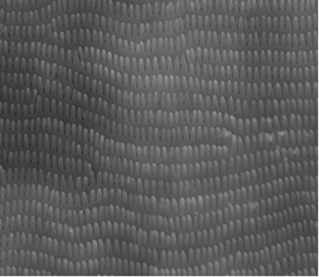
\includegraphics[scale=0.40]{derivation/nanostructuresurface.png}
    \label{fig:nanostruc}
  }
~
  \subfigure[Patch Orientation]{
    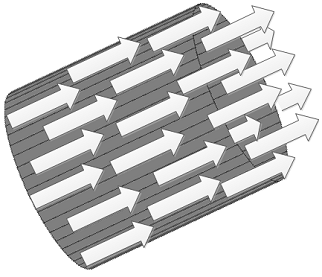
\includegraphics[scale=0.40]{derivation/vectorfieldalongcylinder.png}
    \label{fig:patchvectorfield}
  }
  \caption[Problem Statement]{Input for our simulation}
  \label{fig:problemstatement}
\end{figure}

We want to rely on the integral equation $\ref{eq:mainstam}$ derived by J. Stam in his paper $\cite{diffstam}$ about diffraction shaders. This equation represents a BRDF which models the effect of diffraction caused when a beam of light hits a grating structure. His BRDF is formulated as a function of the Fourier transform of certain correlation functions relating to the given height field. It assumes that the structure of a given grating (i.e. the height field) exhibits a certain degree of regularity. This homogenety assumption of the structure enables him to accurately estimate the correlation function relying on statistical properties of the given height field. However, modelling the complexitiy of a biological nanostrucrue sufficiently and accurately by relying on statistical methods is a non-trivial task. This is why interactive computation at high resolution becomes a hard task, since we cannot evaluate the given integral equation on the fly. Therefore, we have to adapt Stam's equation such that we are able to perform interactive rendering using explicitly provided height fields at interactive rates.

\begin{figure}[H]
  \centering
  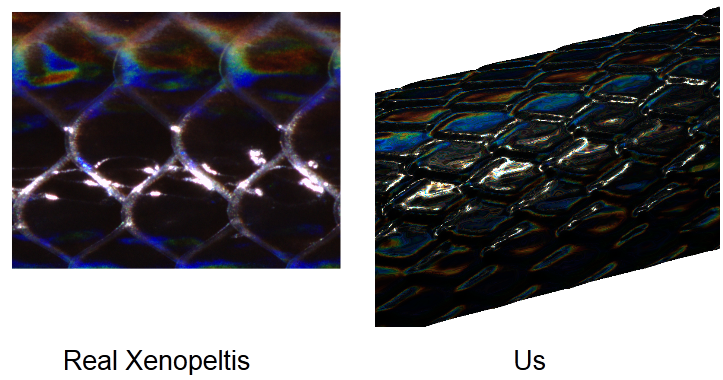
\includegraphics[scale=0.6]{derivation/ourresultswhenrendering.png}
  \caption[Problem Statement: Output]{Output: Rendered Structural Colors}
  \label{fig:problemstatementoutput}
\end{figure}

\section{Approximate a FT by a DFT}
\label{sec:approxftbydft}
Before we will start with our actual adaption of Stam's BRDF model, we first derive some useful identies which are later used during our main derivation in section $\ref{sec:adaptionstambrdfmodel}$. The goal of this section is to provide an approximation of a FT using the DFT when dealing with a bandlimitted signal. For this purpose we will exploit the concept of windowing a function and spatial coherence as described in section $\ref{sec:spatialcoherenceandwindowing}$.

\subsection{Reproduce FT by DTFT}
\label{sec:ftbydtft}
In the following sections, we derive an identity to approximate the FT by the DTFT. This identity will be used to derive the reflected spectral radiance $L_{\lambda}(\omega_r)$ when using Stam's BRDF for a given input height field. However, its expression, which is stated in equation $\ref{eq:nonrelativebrdffinding}$ requires an evaluation of the Fourier transform applied on a given height field$\footnote{actually it requires the computation of the inverse Fourier Transform of a transformed version of the given height field, the function p(x,y) defined in equation \ref{eq:px}.}$ along every possible viewing and light direction. Figure $\ref{fig:ftbydtft}$ visualized the idea of how to obtain the DTFT from the FT for a one dimensional signal$\footnote{For our case we are dealing with a two dimensional, spatial signal, the given height field. Nevertheless, without any constraints of generality, the explained approach applies to multi dimensional problems.}$ \\

\begin{figure}[ht]
  \centering
  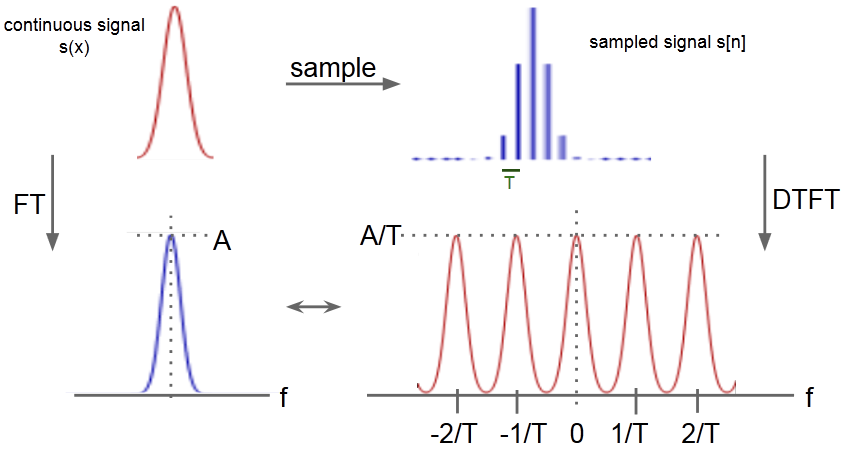
\includegraphics[scale=0.65]{derivation/ftbydtft.png}
  \caption[FT by DTFT]{Illustration of how to approximate the analytical Fourier Transform (FT) $\footnotemark$ of a given continuous signal by a Discrete Time Fourier Transform (DTFT). The DTFT applied on a band-limited, discretized signal yields a continuous, periodic response in frequency space.}
  \label{fig:ftbydtft}  
\end{figure}
\footnotetext{Images of function plots taken from \texttt{http://en.wikipedia.org/wiki/Discrete\textunderscore Fourier\textunderscore transform} and are modified.} 
The first step is to uniformly discretize the given signal since computers are working finite, discrete arithmetic. We rely on the Nyquist–Shannon sampling theorem tells us how dense we have to sample a given signal $s(x)$ such that can be reconstructed its sampled version $\hat{s}[n]$$\footnote{n denotes the number of samples.}$. In particular, a sampled version according to the Nyquist–Shannon sampling theorem will have the same Fourier transform as its original signal when it has a limitted bandwidth. The sampling theorem states that if $f_{max}$ denotes the highest frequency of $s(x)$, then, it has to be sampled by a rate of $f_s$ with $2f_{max} \leq f_s$ in order to be reconstructable. By convention $T = \frac{1}{f_s}$ represent the interval length between two samples. \\ \\

Next, we apply the Fourier transformation operator on the discretized signal $\hat{s}$ which gives us the following expression: 

\begin{align}
\mathcal{F}_{FT}\{\hat{s}\}(w)
& = \int_{\mathds{R}} \hat{s}[n] e^{-iwx} dx \nonumber\\
& = \int_{\mathds{R}} mask(x)s(x) e^{-iwx} dx \nonumber\\
& = T\sum_{x=-\infty}^{\infty} \hat{s}[x] e^{-iwx} \nonumber\\
& = T\mathcal{F}_{DTFT}\{s\}(w)
\label{eq:sampledsignalfttodtft}
\end{align} 
Equation $\ref{eq:sampledsignalfttodtft}$ tells us that if $\hat{s}$ is sufficiently sampled, then its DTFT corresponds to the FT of $s(x)$ . Notice that the resulting DTFT from the sampled signal has a height of $\frac{A}{T}$ where A is the height of the FT of $s$ and thus is a scaled version of the FT. \\

For a given height field $h$, let us compute Stam's auxiliary function $p$ defined as in equation $\ref{eq:px}$. For the reminder of this thesis we introduce the following definition: 

\begin{equation}
  P_{dtft} \equiv \mathcal{F}_{DTFT}\{p\}
\label{eq:dtftheightfield}
\end{equation} 

Therefore $P_{dtft}$ denotes the DTFT of a transformed version of our height field $h$ $\footnote{By transformed height field we mean $p(x,y) = e^{i\frac{2 \pi}{\lambda} w h(x,y)}$ which we get, when we plug $h$ into equation $\ref{eq:heightfieldphase}$ and this expression again plug into equation $\ref{eq:px}$.}$. 

\subsection{Spatial Coherence and Windowing}
\label{sec:spatialcoherenceandwindowing}
Before we can derive a final expression in order to approximate a FT by a DFT, we first have to revisit the concept of coherence introduced in section $\ref{sec:wavecoherence}$ of chapter 2. Previously we have seen that wave-theory tells us what is the total contribution of all secondary sources which allows us to say what is the reflected spectral radiance at a certain point in space. This is related to stationary interference which itself depends on the coherence property of the emitted secondary wave sources. The ability for two points in space, $t_1$ and $t_2$, to interfere in the extend of a wave when being averages over time is the so called spatial coherence. The spatial distance between such two points over which there is significant interference is limited by the quantity coherence area. For filtered sunlight on earth this is equal to 65$\mu m$ $\footnote{A proof for this number can be looked up in the book Optical Coherence and Quantum Optics$\cite{optcoherence}$ on page 153 and 154.}$.

\begin{figure}[H]
  \centering
  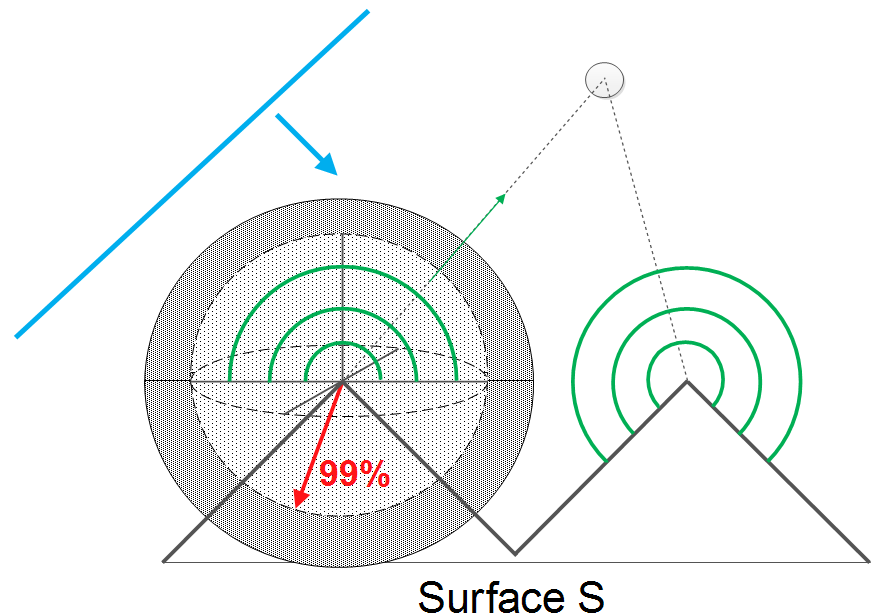
\includegraphics[scale=0.5]{derivation/windowinggaussian.png}
  \caption[Coherence Area using Gaussian Window]{A plane wave encounters a surface. According to Huygens principle, secondary wavelets are emitted of from this surface. The resulting wave at a certain point in space (here indicated by a gray circle) depends on the interference among all waves encountering at this position. The amount of significant interference is directly affected by the spatial coherence property of all the wavelets.}
  \label{fig:coherenceareagaussianwindow}  
\end{figure}

Figure $\ref{fig:coherenceareagaussianwindow}$ illustrates the concept of spatial coherence. A wavefront (blue line) encounters a surface. Due to Huygen's principle, secondary wavelets are emitted off from the surface. The reflected radiance at a certain point in space, e.g. at a viewer's eye position (denoted by the gray circle), is a result of interference among all wavelets at that point. This interference is directly affected by the spatial coherence property of all the emitted wavelets. \\

In physics spatial coherence is predicted by the cross correlation between $t_1$ and $t_2$ and usually modelled by a Gaussian Random Process. For any such Gaussian Process we can use a spatial gaussian window $g(x)$ which is equal:

\begin{equation} 
  g(x) = \frac{1}{\sqrt{2\pi}\cdot\sigma}\cdot e^{-\frac{x^2}{2\sigma^2}} 
  \label{eq:gaussianwindowspacial}
\end{equation} 

We have chosen standard deviation $\sigma_s$ of the window such that it fulfills the equation $4 \sigma_s = 65\mu m$. This is equivalent to saying that we want to predict about $99.99\%$$\footnote{Standard deviation values from confidence intervals table of normal distribution provided by Wolfram MatheWorld \texttt{http://mathworld.wolfram.com/StandardDeviation.html}.}$ of the resulting spatial coherence interference effects in our model by a cross correlation function. \\

By applying the Fourier transformation to the spatial window we get the corresponding window in frequency space as:
\begin{equation} 
  G(f) = e^{-\frac{f^2}{2\sigma_f^2}}
  \label{eq:gaussianwindowfrequencyspace}
\end{equation} 

Notice that this frequency space window has a standard deviation $\sigma_f$ equal to $\frac{1}{2 \pi \sigma_s}$. Those two windows, the spatial- and the frequency space window, will be used in the next section in order to approximate the DTFT by the DFT by a windowing approach.

\subsection{Reproduce DTFT by DFT}
\label{sec:gaussianwindow}

In this section we explain how and under what assumptions the DTFT of a discretized signal$\footnote{E.g. a sampled signal like already presented in figure $\ref{fig:ftbydtft}$}$ can be approximated by a DFT. The whole idea how to reproduce the DTFT by DFT is schematically illustrated in figure $\ref{fig:dtftbydft}$.

\begin{figure}[H]
  \centering
  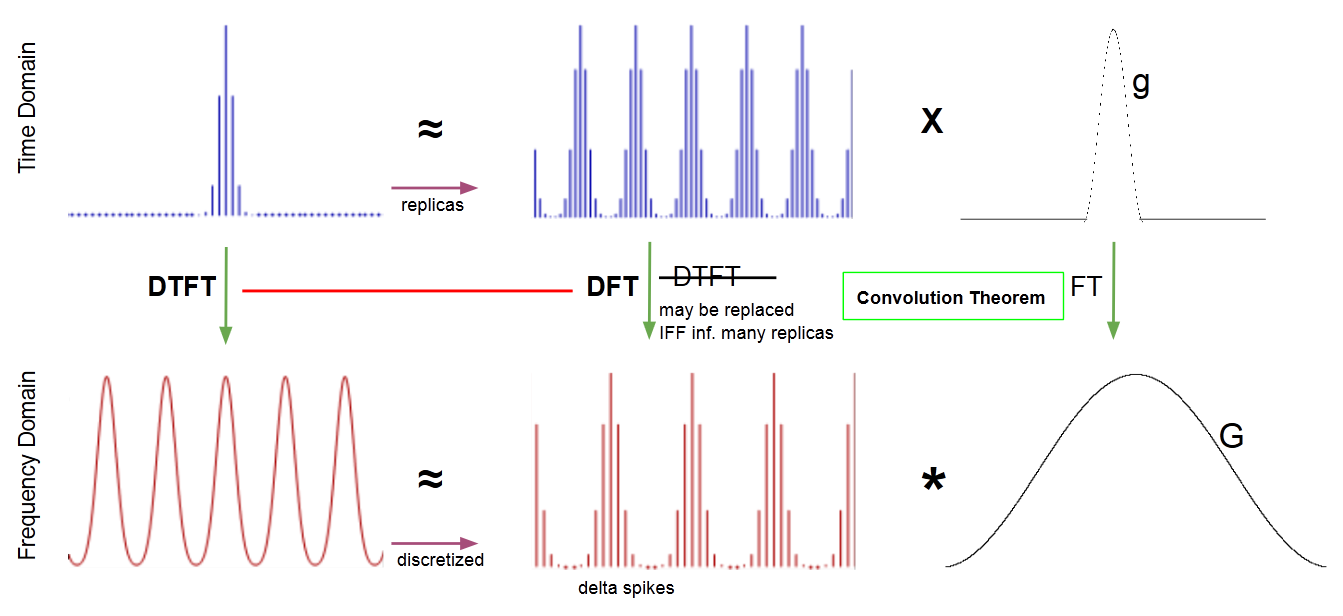
\includegraphics[scale=0.45]{derivation/dtftbydft.png}
  \caption[DTFT by DFT]{Illustration of how to approximate the DTFT $\footnotemark$ by the DFT relying on the Convolution Theorem, using a gaussian window function.}
  \label{fig:dtftbydft}  
\end{figure}
\footnotetext{Images of function plots taken from \texttt{http://en.wikipedia.org/wiki/Discrete\textunderscore Fourier\textunderscore transform} and are modified. Note that the scales in the graphic are not appropriate.} 

Lets say, we are given a spatial, band-limited and discretized one dimensional signal $\hat{s}$. Our goal is to approximate this spatial signal in a way such that when taking the DFT of this approximated signal, it will yield the same response as taking the DTFT of the original sampled $\hat{s}$. For this purpose we will use the previously introduced concept of gaussian windows and the so called Convolution Theorem which is a fundamental property of all Fourier transformations. \\

The Convolution Theorem states that the Fourier transformation of a product of two functions, $f$ and $g$, is equal to convolving the Fourier Transformations of each individual function. Mathematically, this statement corresponds to equation $\ref{eq:convolutiontheorem}$:

\begin{equation} 
  \mathcal{F}\{f\cdot g\} = \mathcal{F}\{f\} * \mathcal{F}\{g\}
  \label{eq:convolutiontheorem}
\end{equation}

The principal issue is how to approximate our given signal $\hat{s}$. Therefore, let us consider another signal $\hat{s_N}$ which is the $N$ times replicated version of $\hat{s}$ (blue signal at center top in figure). \\

Remember that, in general, the wave magnitude at a certain point in space is the result of interference among all wavelength meeting at that position. In our scenario, the source of those signals are emitted secondary wavelets. The interference strength between wavelets is related to their spatial coherence. Windowing the signal by a gaussian window $g$ is akin to modelling the effects of spatial coherence interference on the surface. From the previous section $\ref{sec:spatialcoherenceandwindowing}$ we know that we can use gaussian window like in equation $\ref{eq:gaussianwindowspacial}$ in order to approximate such spatial signals interference effects. \\

Using this insight, we can approximate $\hat{s}$ by taking the product of $\hat{s_N}$ with a gaussian window $g$. This fact is illustrated in the first row of figure $\ref{fig:ftbydtft}$. So, what will the DTFT of this approximation yield? We already know that the DTFT of $\hat{s}$ is a continuous, periodic signal, since $\hat{s}$ is band-limited. Thus, taking the DTFT of this found approximation should give us approximatively the same continuous, periodic signal. \\

This is where the convolution theorem comes into play: Applying the DTFT to the product of $\hat{s_N}$ and $g$ is the same as convolving the DTFT of $\hat{s_N}$ by DTFT of $g$. From equation $\ref{eq:gaussianwindowfrequencyspace}$ we already know that the DTFT of $g$ is just another gaussian, denoted by $G$. On the other hand the DTFT of $\hat{s_N}$ yields a continuous, periodic signal. The higher the value of N, the sharper the signal gets (denoted by delta spiked) and the closer it converges toward to the DFT. This is why the DFT is the limit of a DTFT applied on periodic and discrete signals. Therefore, for a large number of $N$ we can replace the DTFT by the DFT operator when applied on $\hat{s_N}$. \\

Lastly, we see that the DTFT of $\hat{s}$ is approximately the same like convolving a gaussian window by the DFT of $\hat{s_N}$. This also makes sense, since convolving a discrete, periodic signal (DFT of $\hat{s_N}$) by a continuous window function $G$ yields a continuous, periodic function. \\

In general, for every non-windowed signal, we cannot compute its DTFT $\ref{eq:dtft}$ numerically due to finite computer arithmetic and hence working with the DFT is our only option. Furthermore, there are numerically fast algorithms in order to compute the DFT values of a function, the Fast Fourier Transformation (FFT). The DFT $\ref{eq:dft}$ of a discrete height field is equal to the DTFT of an infinitely periodic function consisting of replicas of the same height field. Now, let a spatial gaussian window $g$ having a standard deviation for which $4\sigma_s$ is equal 65$\mu m$. Then, from before, it follows:

\begin{equation}
\mathcal{F}_{dtft}\{\mathbf{s}\} \equiv \mathcal{F}_{dft} \{\mathbf{s}\} * G(\sigma_f)
\end{equation} 

Therefore we can deduce the following expression:

\begin{align}
\mathcal{F}_{dtft} \{\mathbf{t}\}(u,v)
& = \int_{-\infty}^{\infty} \int_{-\infty}^{\infty} {F}_{dft}\{\mathbf{t}\}(w_u,w_v) \phi(u-w_u, v-w_v) dw_u dw_v \nonumber \\
& = \int_{-\infty}^{\infty} \int_{-\infty}^{\infty} \sum_i \sum_j {F}_{dft} \{\mathbf{t}\}(w_u,w_v) \nonumber \\ 
& \quad \quad \delta(w_u-w_i, w_v-w_j)\phi(u-w_u, v-w_v) dw_u dw_v \nonumber \\
& = \sum_i \sum_j \int_{-\infty}^{\infty} \int_{-\infty}^{\infty}  {F}_{dft} \{\mathbf{t}\}(w_u,w_v) \nonumber \\
& \quad \quad \delta(w_u-w_i, w_v-w_j)\phi(u-w_u, v-w_v) dw_u dw_v \nonumber \\
& = \sum_i \sum_j {F}_{dft} \{\mathbf{t}\}(w_u,w_v) \phi(u-w_u, v-w_v)
\end{align}

where 

\begin{equation} 
 \phi(x,y) = \pi e^{-\frac{x^2 + y^2}{2\sigma_{f}^2}}
  \label{eq:gaussweight}
\end{equation} 

\section{Adaption of Stam's BRDF for Discrete Height Fields}
\label{sec:adaptionstambrdfmodel}
Our goal is to render structural colors using Stam's BRDF$\footnote{Remember that a BRDF is the portion of a incident light source reflected off a given surface towards a specified viewing direction.}$ using natural gratings. According to our problem statement stated in section $\ref{sec:problemstatement}$ we have to reformulate his BRDF equation. We will end up with an identity of the reflected spectral radiance. This is where the rendering equation from section $\ref{sec:renderingequation}$ comes into play. Having looked at some basic derivations from section $\ref{sec:approxftbydft}$ we start our adaption of Stam's BRDF model in the following sections.

\subsection{Reflected Radiance of Stam's BRDF}
We are going to use Stam's main derivation $~\eqref{eq:mainstam}$ for the $BRDF(\omega_i, \omega_r)$ in $\ref{eq:deribrdfwithdirsource}$ by applying the fact that the wavenumber is equal $k=\frac{2\pi}{\lambda}$:

\begin{align}
BRDF(\omega_i, \omega_r) 
& = \frac{k^2 F^2 G}{4\pi^2 A w^2} \langle \left|P(ku, kv) \right|^2\rangle \nonumber\\
& = \frac{4 \pi^2 F^2 G}{4\pi^2 A \lambda^2 w^2} \langle \left|P(ku, kv)  \right|^2\rangle \nonumber\\
& = \frac{F^2 G}{A \lambda^2 w^2} \langle \left|P(\frac{2\pi u}{\lambda}, \frac{2\pi v}{\lambda})  \right|^2\rangle
\label{eq:minoradaptedstam}
\end{align}

Going back to equation $\ref{eq:deribrdfwithdirsource}$ and plugging equation $\ref{eq:minoradaptedstam}$ into it, using the definition of equation $\ref{eq:geometricterm}$ and the equation $\ref{eq:sphericalomega}$ for $\omega$ we will get the following:

\begin{align}
L_{\lambda}(\omega_r) 
& = \frac{F^2 (1 + \omega_i \cdot \omega_r)^2}{A \lambda^2 cos(\theta_i)cos(\theta_r)  \omega^2} \left \langle \left|P \left( \frac{2\pi u}{\lambda}, \frac{2\pi v}{\lambda}\right) \right|^2 \right \rangle cos(\theta_i) I(\lambda) \nonumber \\
& = I(\lambda) \frac{F^2 (1 + \omega_i \cdot \omega_r)^2}{\lambda^2 A \omega^2 cos(\theta_r)} \left \langle \left|P \left( \frac{2\pi u}{\lambda}, \frac{2\pi v}{\lambda}\right) \right|^2 \right \rangle
\label{eq:nonrelativebrdffinding}
\end{align}

Note that the Fresnel term $F$ is actually a function of $(w_i, w_r)$, but in order to keep the equations simple, we omitted its arguments. \\

So far we just plugged Stam's BRDF identity into the rendering equation and hence have not deviated from his formulation. Keep in mind that $P$ denotes the Fourier transformation of a given discrete height field. Its FT depends on the viewing and incidence light direction. Thus this Fourier transform has to be recomputed for every direction which will slow down the whole computation quite a lot$\footnote{Even a fast variant of computation for the two dimensional Fourier transform has a runtime complexity of $O\left( N^2 \log{N}\right)$ for a N by N discretized signal.}$. According to section $\ref{sec:ftbydtft}$, when applying the Fourier transformation to a discrtized function, we have to apply the DTFT operator. Thus when interested in computing the Fourier tranformation of a given discrete height field, we have to apply the DTFT operator to it. One particular strategy to solve this issue is to approximate $P$ by the Discrete Fourier Transform (DFT)$\footnote{See appendix \ref{chap:appendixsignalprocessing} for further information about different kinds of Fourier transformations.}$ and separate its computation such that terms for many directions can be precomputed and then later retrieved by look ups. For the approximation of $P$ we rely on the derivations from section $\ref{sec:approxftbydft}$. Firtly, we approximated the FT by DTFT and then we approximated the DTFT by the DFT. For the basics of signal processing and Fourier transformations please refer the appendix $\ref{chap:appendixsignalprocessing}$. \\

Using the insight gained by equation $\ref{eq:sampledsignalfttodtft}$ allows us to further simplify equation $\ref{eq:nonrelativebrdffinding}$:

\begin{align}
L_{\lambda}(\omega_r) 
& = I(\lambda) \frac{F^2 (1 + \omega_i \cdot \omega_r)^2}{\lambda^2 A w^2 cos(\theta_r)} \left \langle \left|P \left( \frac{2\pi u}{\lambda}, \frac{2\pi v}{\lambda}\right) \right|^2 \right \rangle \nonumber \\
& = I(\lambda) \frac{F^2 (1 + \omega_i \cdot \omega_r)^2}{\lambda^2 A w^2 cos(\theta_r)} \left \langle \left|T^2 P_{dtft}\left( \frac{2\pi u}{\lambda}, \frac{2\pi v}{\lambda}\right) \right|^2 \right \rangle
\label{eq:nonrelativebrdffindingreproddtft}
\end{align}

Where $P_{dtft}$ is a substitute for $\mathcal{F}_{DTFT}\{p\}(w)$. Furthermore $T$ the sampling distance for the discretization of $p(x,y)$ assuming equal and uniform sampling along both $x$ and $y$ dimensions.

\subsection{Relative Reflectance}
\label{sec:relrefl}
In this section we are going to explain how to scale our BRDF formulation such that all of its possible output values are mapped into the range $\left[0,1\right]$. Such a relative reflectance formulation will ease our life for later rendering purposes since usually color values are within the range $\left[0,1\right]$, too. Furthermore, this will allow us to properly blend the resulting illumination caused by diffraction with a texture map. \\

Let us examine what $L_\lambda(\omega_r)$ will be for a purely specular surface, for which $\omega_r = \omega_0 = \omega_i$ such that $\omega_0 = (0,0,1)$. For this specular reflection case, the corresponding radiance will be denoted as $L_\lambda^{spec}(\omega_0)$. We define the relative reflected radiance for our problem $\ref{eq:nonrelativebrdffinding}$ by simply taking the fraction between $L_\lambda(\omega_r)$ and $L_\lambda^{spec}(\omega_0)$ which is denoted by: 

\begin{equation}
  \rho_\lambda(\omega_i,\omega_r) = \frac{L_\lambda(\omega_r)}{L_\lambda^{spec}(\omega_0)}
  \label{eq:rohrel}
\end{equation}

Notice that the third component $w$ from the vector in equation $\ref{eq:uvw}$ is squared equal to $(cos(\theta_i)+cos(\theta_r))^2$$\footnote{Consult section $\ref{sec:componentw}$ in the appendix}$. But first, let us derive the following expression:

\begin{align}
L_\lambda^{spec}(\omega_0) 
& = I(\lambda) \frac{F(\omega_0, \omega_0)^2 (1+\colvec[0]{0}{1}\cdot\colvec[0]{0}{1})^2}{\lambda^2 A (cos(0)+cos(0))^2 cos(0)} \langle \left|T_0^2 P_{dtft}(0,0)  \right|^2\rangle \nonumber \\
& = I(\lambda) \frac{F(\omega_0, \omega_0)^2 (1+1)^2}{\lambda^2 A (1+1)^2 1}\left| T_0^2 N_{sample} \right|^2 \nonumber \\
& = I(\lambda) \frac{F(\omega_0, \omega_0)^2}{\lambda^2 A}\left| T_0^2 N_{sample} \right|^2 
\label{eq:lspec}
\end{align}

Where $N_{samples}$ is the number of samples of the DTFT $\ref{eq:dtft}$. Thus, we can plug our last derived expression $\ref{eq:lspec}$ into the definition for the relative reflectance radiance $\ref{eq:rohrel}$ in the direction $w_r$ and we get:

\begin{align}
\rho_\lambda(\omega_i,\omega_r)
& = \frac{L_\lambda(\omega_r)}{L_\lambda^{spec}(\omega_0)} \nonumber \\
& = \frac{I(\lambda) \frac{F(\omega_i, \omega_r)^2 (1 + \omega_i \cdot \omega_r)^2}{\lambda^2 A (cos(\theta_i)+cos(\theta_r))^2 cos(\theta_r)} \langle \left|T_0^2 P_{dtft}(\frac{2\pi u}{\lambda}, \frac{2\pi v}{\lambda}) \right|^2\rangle}{I(\lambda) \frac{F(\omega_0, \omega_0)^2}{\lambda^2 A}\left| T_0^2 N_{sample} \right|^2 } \nonumber \\
& = \frac{F^2(\omega_i,\omega_r)(1 + \omega_i \cdot \omega_r)^2}{F^2(\omega_0,\omega_0)(cos(\theta_i)+cos(\theta_r))^2 cos(\theta_r)} \langle \left|\frac{P_{dtft}(\frac{2\pi u}{\lambda}, \frac{2\pi v}{\lambda})}{N_{samples}}\right|^2\rangle
\label{eq:lspecrohrel}
\end{align}

For simplification and better readability, let us define the following gain-factor:

\begin{equation} 
    C(\omega_i,\omega_r) = \frac{F^2(\omega_i,\omega_r)(1 + \omega_i \cdot \omega_r)^2}{F^2(\omega_0,\omega_0)(cos(\theta_i)+cos(\theta_r))^2 cos(\theta_r) N_{samples}^2}
\label{eq:cfact}
\end{equation}

Using equation $\ref{eq:cfact}$, we get the following expression for the relative reflectance radiance from equation $\ref{eq:lspecrohrel}$:

\begin{equation}
\rho_\lambda(\omega_i,\omega_r) =  C(\omega_i,\omega_r) \langle \left|P_{dtft}(\frac{2\pi u}{\lambda}, \frac{2\pi v}{\lambda})\right|^2\rangle
\label{eq:cpterm}
\end{equation}

Using the previous definition for the relative reflectance radiance equation $\ref{eq:rohrel}$:

\begin{equation}
 \rho_\lambda(\omega_i,\omega_r) = \frac{L_\lambda(\omega_r)}{L_\lambda^{spec}(\omega_0)} \nonumber
\end{equation}

which we can rearrange to the expression: 

\begin{equation}
L_\lambda(\omega_r) = \rho_\lambda(\omega_i,\omega_r)L_\lambda^{spec}(\omega_0)
\label{eq:radianceomegarspec}
\end{equation}

Let us choose $L_\lambda^{spec}(w_0) = S(\lambda)$ such that is has the same profile as the relative spectral power distribution of CIE Standard Illuminant $D65$ (discussed in $\ref{subsec:colortransformations}$). Furthermore, when integrating over $\lambda$ for a specular surface, we should get $CIE_{XYZ}$ values corresponding to the white point for $D65$. The corresponding tristimulus values using CIE colormatching functions $\ref{eq:tristimulusvalues}$ for the $CIE_{XYZ}$ values look like:

\begin{align}
X = \int_{\lambda}L_\lambda(\omega_r)\overline{x}(\lambda)d\lambda \nonumber \\
Y = \int_{\lambda}L_\lambda(\omega_r)\overline{y}(\lambda)d\lambda \nonumber \\
Z = \int_{\lambda}L_\lambda(\omega_r)\overline{z}(\lambda)d\lambda
\label{eq:tristimrad}
\end{align}

where $\overline{x}$, $\overline{y}$, $\overline{z}$ are the color matching functions. Combining our last finding from equation $\ref{eq:radianceomegarspec}$ for $L_\lambda(\omega_r)$ with the definition of the tristimulus values from equation $\ref{eq:tristimrad}$, allows us to 
derive a formula for computing the colors values using Stam's BRDF formula relying on the rendering equation $\ref{eq:initialbrdf}$. Without any loss of generality it suffices to derive an explicit expression for just one tristimulus term, for example Y, the luminance:

\begin{align}
Y 
& =\int_{\lambda}L_\lambda(\omega_r)\overline{y}(\lambda)d\lambda \nonumber \\
& =\int_{\lambda}\rho_\lambda(\omega_i,\omega_r)L_\lambda^{spec}(\omega_0) \overline{y}(\lambda)d\lambda \nonumber \\
& =\int_{\lambda}\rho_\lambda(\omega_i,\omega_r) S(\lambda) \overline{y}(\lambda)d\lambda \nonumber \\
& =\int_{\lambda} C(\omega_i,\omega_r) \langle \left|P_{dtft}(\frac{2\pi u}{\lambda}, \frac{2\pi v}{\lambda})\right|^2\rangle S(\lambda) \overline{y}(\lambda)d\lambda \nonumber \\
& = C(\omega_i,\omega_r) \int_{\lambda} \langle \left|P_{dtft}(\frac{2\pi u}{\lambda}, \frac{2\pi v}{\lambda})\right|^2\rangle S(\lambda) \overline{y}(\lambda)d\lambda \nonumber \\
& = C(\omega_i,\omega_r) \int_{\lambda} \langle \left|P_{dtft}(\frac{2\pi u}{\lambda}, \frac{2\pi v}{\lambda})\right|^2\rangle S_y(\lambda)d\lambda
\label{eq:structuralcolorsslow}
\end{align}

Where we used the definition $S_y(\lambda)\overline{y}(\lambda)$ in the last step.

\section{Optimization using Taylor Series}
\label{sec:taylorapproximation}
Our final goal is to render structural colors resulting by the effect of wave diffraction. So far, we have derived an expression which can be used for rendering. Nevertheless, our current equation $\ref{eq:structuralcolorsslow}$ used for computing structural colors, cannot directly be used for interactive rendering, since $P_{dtft}$ had do be recomputed for every change in any direction$\footnote{According to changes in viewing- or incident light direction.}$. \\

In this section, we will address this issue and deliver an approximation for $P_{dtft}$ defined in equation $\ref{eq:dtftheightfield}$.
This approximation will allow us to separate $P_{dtft}$ in a certain way such that some computional expensive terms can be precomputed. The main idea is to formulate $P_{dtft}$ as a series expansion relying on the definition of Taylor Series, as defined in equation $\ref{eq:deftaylor}$. Further, we will provide an error bound for our approximation approach for a given number of terms. Lastly, we will substitute our approximation into our BRDF formula from equation $\ref{eq:structuralcolorsslow}$. \\

Let us consider $p(x,y)=e^{ikwh(x,y)}$ form Stam's Paper $\ref{sec:sumstam}$ where $h(x,y)$ is a given height field and $k = \frac{2 \pi}{\lambda}$ denotes the wavenumber of wavelength $\lambda$. For any complex number $t$ the power series expansion of the exponential function is equal to:
 
\begin{equation}
  e^{t}=1+t+\frac{t^{2}}{2!}+\frac{t^{3}}{3!}+...=\sum_{n=0}^{\infty}\frac{t^{n}}{n!}
  \label{eq:expseriesexpansion}
\end{equation}

Now, when we use the exponent$\footnote{This exponent is a complex valued function, equal to ikwh(x,y).}$ of $p(x,y)$ as an input argument for equation $\ref{eq:expseriesexpansion}$ we get:

\begin{align}
 e^{t}
 &=e^{ikwh} \nonumber \\
 &=1+(ikwh)+\frac{1}{2!}(ikwh)^{2}+\frac{1}{3!}(ikwh)^{3}+... \nonumber \\
 &=\sum_{n=0}^{\infty}\frac{(ikwh)^{n}}{n!}.
 \label{eq:expseriesexpr}
\end{align}

where $i$ is the imaginary unit for complex numbers. For simplification, in the reminder of this section we omitted the arguments of $h$. Equation $\ref{eq:expseriesexpr}$ gives us an expression for an exponential series expansion for the exponent of $p(x,y)$. Please note that the above Taylor series is convergent for any complex valued number. Therefore the equation $\ref{eq:expseriesexpr}$ is equal to

\begin{equation}
  p(x,y)=\sum_{n=0}^{\infty}\frac{(ikwh(x,y))^{n}}{n!}
  \label{eq:pxyseries}
\end{equation}

and thus gives us a series representation of $p(x,y)$. Next, calculating the Fourier transformation $\mathcal{F}$ of equation $\ref{eq:pxyseries}$ gives us the identity:

\begin{align}
  \mathcal{F}\left\{ p\right\}
  & \equiv \mathcal{F}\left\{ \sum_{n=0}^{\infty}\frac{(ikwh)^{n}}{n!}.\right\} \nonumber \\
  & \equiv \sum_{n=0}^{\infty}\mathcal{F}\left\{ \frac{(ikwh)^{n}}{n!}\right\} \nonumber \\
  & \equiv \sum_{n=0}^{\infty}\frac{(ikw)^{n}}{n!}\mathcal{F}\left\{ h{}^{n}\right\}
  \label{eq:ftlinopid}
\end{align}

Where we have exploited the fact that the Fourier transformation is a linear operator. Therefore, in equation $\ref{eq:ftlinopid}$, we have shown that the Fourier transformation of a series is equal to the sum of the Fourier transformation, applied on each individual series term. Reusing the identifier $P$$\footnote{This identifier P may be subscripted by \emph{dtft} which will denote the DTFT variant of P.}$ in order to determine the Fourier transformation of $p$ from equation $\ref{eq:px}$ equation $\ref{eq:ftlinopid}$ then correspond to:

\begin{equation}
  P(\alpha,\beta)=\sum_{n=0}^{\infty}\frac{(ikw)^{n}}{n!}\mathcal{F}\left\{ h{}^{n}\right\} (\alpha,\beta)
\end{equation}

Up to now we have found a infinity series representation for $P_{dtft}$. Next we are going to look for an upper bound $N\mathbb{\in N}$ such that 

\begin{align}
  \tilde{P}_{N}(\alpha,\beta)
  :=\sum_{n=0}^{N}\frac{(ikwh)^{n}}{n!}\mathcal{F}\left\{ h{}^{n}\right\} (\alpha,\beta)
  \approx P(\alpha,\beta)
  \label{eq:taylorseriesapproximationofp} 
\end{align}

$\tilde{P}_{N}$ is a good approximation of $P$, i.e. their absolute difference is small$\footnote{Mathematically speaking, this statement correspond to $|| \tilde{P}_{N} - P|| \leq \epsilon$, where $\epsilon$ > 0 is a small number.}$. But first, the following two facts would have to be proven$\footnote{Please have a look in section $\ref{chap:taylorseriesapproxappendix}$ in the appendix}$:

\begin{enumerate}
\item Show that there exist such an $N\mathbb{\in N}$ s.t. the approximation of equation $\ref{eq:taylorseriesapproximationofp}$ holds true.
\item Find a value for $N$ s.t. this approximation is below a certain error bound, e.g. close to machine precision $\epsilon$. 
\end{enumerate}

Our facts are valid and proven (see appendix $\ref{chap:taylorseriesapproxappendix}$) implies that there actually exists such an $N$. Thus, we can make use of the taylor series approximation from equation $\ref{eq:taylorseriesapproximationofp}$ and use it for approximating $P_{dtft}$. This idea allows us to adapt equation $\ref{eq:structuralcolorsslow}$, which is used for computing the structural colors of our BRDF model, in a numerically fast way. Finally the equation for the luminance is equal to:

\begin{align}
Y 
& = C(w_i,w_r) \int_{\lambda} \langle \left|P_{dtft}(\frac{2\pi u}{\lambda}, \frac{2\pi v}{\lambda})\right|^2\rangle S_y(\lambda)d\lambda \nonumber \\
& = C(w_i,w_r) \int_{\lambda} \left| \sum_{n=0}^N \frac{(wk)^n}{n!} \mathcal{F}\{i^n h^n\}(\frac{2\pi u}{\lambda}, \frac{2\pi v}{\lambda})\right|^2 S_y(\lambda)d\lambda
\label{eq:xcolexpression}
\end{align}

Notice that equation $\ref{eq:xcolexpression}$ is constrained by $N$ and hence is an approximation of equation $\ref{eq:structuralcolorsslow}$. Furthermore, it is possible to seperate out all the Fourier Terms in the summation and precompute them. This is why the approach in equation $\ref{eq:xcolexpression}$ is fast in order to compute structural color values according to our BRDF model. In other words this means that the Fourier terms in equation $\ref{eq:xcolexpression}$ are not anymore dependent on $\omega$ when using this Taylor series approximation.

\section{Spectral Rendering using DFTs}
\label{sec:spectralrendering}
In this section we describe how our final model for rendering structural colors due to diffraction will look like. For this purpose we use all our previous findings and plug them together to one big equation. For a given height field $h$ representing the surface of a grating, we want to compute the resulting color due to light diffracted on that grating. For rendering we rely on the $CIE_{XYZ}$ colorspace. For given direction vectors $w_i$ and $w_r$ as shown in figure $\ref{fig:geometricsetup}$ the DFT of the height field is equal to:

\begin{equation}
DFT_{n}\{h\}(u,v) = {F}_{dft}\{i^n h^n\}(\frac{2\pi u}{\lambda},\frac{2\pi v}{\lambda})
\label{eq:subdfteq}
\end{equation}

From section $\ref{sec:gaussianwindow}$ we know that we can reproduce a FT by applying a Gaussin window on the DFT from equation $\ref{eq:subdfteq}$. This windowing approach gives us: 

\begin{equation}
  W_{n}(u,v) = \sum_{(r,s) \in \mathcal{N}_1(u,v)} \left| DFT_{n}\{h\}(u-w_r, v-w_s) \right|^2 \phi(u-w_r, v-w_s)
  \label{eq:wnwindowingapproachsub}
\end{equation}

where $\phi(x,y) = \pi e^{-\frac{x^2 + y^2}{2\sigma_{f}^2}}$ is the Gaussian window from equation $\ref{sec:gaussianwindow}$ and $\mathcal{N}_1(u,v)$ denotes an the k-ring neighborhood around $(u,v)$ with k as a parameter. \\

In section $\ref{sec:taylorapproximation}$ we derived equation $\ref{eq:xcolexpression}$ which tells us how to compute the $CIE_{XYZ}$ color value of a particular color channel using our relative reflectance BRDF model from section $\ref{sec:relrefl}$. Plugging all these findings together and using our windowing approach, listed in equation $\ref{eq:wnwindowingapproachsub}$, Then $\forall (u,v,w)$ like (defined in equation $\ref{eq:uvw}$), our final expression for computing structural colors due to diffraction, using all our previous derivations, will be equal:

\begin{equation}
\begin{split}
\colvec[X]{Y}{Z}& = C(\omega_i,\omega_r) \int \limits_{\Lambda} \sum_{n=0}^N  \frac{(2 \pi w)^n}{\lambda^n n!} W_{n}(u,v) \colvec[S_x(\lambda)]{S_y(\lambda)}{S_z(\lambda)}d\lambda
\end{split}
\label{eq:finalexpression}
\end{equation}

Where $C(\omega_i,\omega_r)$ is the defined in equation $\ref{eq:cfact}$. Note that equation $\ref{eq:finalexpression}$ integrates over a given wavelength spectrum, denoted by $\Lambda$. Usually, this $\Lambda$ is equal to $[\lambda_{min}, \lambda_{max}]$ where $\lambda_{min} = 380nm$ and $\lambda_{max}=780nm$. \\

\section{An Alternative Approach}
\subsection{PQ factors}
\label{sec:pq}
In this section we are presenting an alternative approach to the previous Gaussian window approach described in section $\ref{sec:gaussianwindow}$ in order to solve the issue of working with the $DTFT$ instead of $DFT$. We assume, that a given surface $S$ is covered by a number of replicas of a provided representative surface patch $f$. In a simplified, one dimensional scenario, mathematically speaking, $f$ is assumed to be a repetitive function, i.e. $\forall x \in \mathds{R} : S(x) = S(x+nT)$, where $T$ is its fundamental period and $n \in \mathds{N}_{0}$. Thus, the surfaces can be written formally as:

\begin{equation}
  S(x) = \sum_{n=0}^N f(x+nT)
\label{eq:replicatedpatchsurface}
\end{equation}

What we are looking for is an identity for the Fourier transform$\footnote{Remember that we are using the definition of Fourier Transform used in electrical engineering where $\mathcal{F}$ actually corresponds to the inverse Fourier Transform.}$ of our surface $S$, required in order to simplify the $(X,Y,Z)$ colors from $\ref{eq:xcolexpression}$:

\begin{align}
\mathcal{F}\{S\}(w)
& =\int f(x) e^{iwx}dx \nonumber \\
& =\int_{-\infty}^{\infty} \sum_{n=0}^{N} f(x+nT) e^{iwx}dx \nonumber \\
& =\sum_{n=0}^{N} \int_{-\infty}^{\infty} f(x+nT) e^{iwx}dx
\label{eq:pqsinit}
\end{align}

Next, apply the following substitution $x+nT = y$ which will lead us to:

\begin{gather}
x=y-nT \nonumber \\
dx=dy
\label{eq:substitude1dpq}
\end{gather} 

Plugging this substitution back into equation $\ref{eq:pqsinit}$ we will get: 

\begin{align}
\mathcal{F}\{S\}(w)
& =\sum_{n=0}^{N} \int_{-\infty}^{\infty} f(x+nT) e^{iwx}dx \nonumber \\
& =\sum_{n=0}^{N} \int_{-\infty}^{\infty} f(y) e^{iw(y-nT)}dy \nonumber \\
& =\sum_{n=0}^{N} e^{-iwnT} \int_{-\infty}^{\infty} f(y) e^{iwy}dy \nonumber \\
& =\sum_{n=0}^{N} e^{-iwnT} \mathcal{F}\{f\}(w) \nonumber \\
& =\mathcal{F}\{f\}(w) \sum_{n=0}^{N} e^{-iwnT}
\label{eq:pqsub}  
\end{align}

We used the fact that the exponential term $e^{-iwnT}$ is a constant factor when integrating along $dy$ and the identity for the Fourier Transform of the function $f$. Next, let us examine the series $\sum_{n=0}^N e^{-iwnT}$ closer:

\begin{align}
\sum_{n=0}^N e^{-iwnT}
& =\sum_{n=0}^N (e^{-iwT})^n \nonumber \\
& =\frac{1-e^{iwT(N+1)}}{1-e^{-iwT}}
\label{eq:pqgeometricseries}
\end{align}

We recognize the geometric series identity for the left-hand-side of equation $\ref{eq:pqgeometricseries}$. Mainly relying on trigonometric identities, equation $\ref{eq:pqsub}$ can be further simplified to:  

\begin{align}
\mathcal{F}\{S\}(w)
& = (p+iq) \mathcal{F}\{f\}(w)  
\label{eq:mainfinding1d}
\end{align}

where $p$ and $q$ are defined as:

\begin{align}
p& =\frac{1}{2}+\frac{1}{2}\left(\frac{cos(wTN)-cos(wT(N+1))}{1-cos(wT)}\right) \nonumber \\
q& =\frac{sin(wT(N+1))-sin(wTN)-sin(wT)}{2(1-cos(wT))}
\end{align}

Please notice, all derivation steps can be found in the appendix in section $\ref{sec:pqonedimappendix}$. \\

Now lets consider our actual problem description. Given a patch of a nano-scaled surface snake shed represented as a two dimensional height field $h(x,y)$. We once again assume that this provided patch is representing the whole surface $S$ of our geometry by some number of replicas of itself. Therefore, $S(x,y) = \sum_{n=0}^{N} h(x+nT_1, y+mT_2)$, assuming that the given height field has the dimensions $T_1$ by $T_2$. In order to derive an identity for the two dimensional Fourier transformation of $S$ we can similarly proceed like we did to derive equation $\ref{eq:mainfinding1d}$.

\begin{align}
\mathcal{F}\{S\}(w_1, w_2)
& =(p + iq) \mathcal{F}_{DTFT}\{h\}(w_1,w_2)
\label{eq:pqmainfinding}
\end{align}

Note that a detailed derivation of equation $\ref{eq:pqmainfinding}$ can be found in the appendix in section $\ref{sec:pqtwodimappendix}$ and we have defined :

\begin{align}
p := (p_1 p_2 - q_1 q_2) \nonumber \\ 
q := (p_1 p_2 + q_1 q_2)
\label{eq:pqsubst2}
\end{align}

For the identity of equation $\ref{eq:pqmainfinding}$ we made use of Green's integration rule which allowed us to split the double integral to the product of two single integrations. Also, we used the definition of the 2-dimensional inverse Fourier transform of the height field function. We applied a similar substitution like we did in $\ref{eq:substitude1dpq}$, but this time twice, once for $x_1$ and once for $x_2$ separately. The last step in equation $\ref{eq:pqmainfinding}$, substituting with $p$ and $q$ in equation $\ref{eq:pqsubst2dappendix}$ will be useful later in the implementation. The insight should be, that the product of two complex numbers is again a complex number. We will have to compute the absolute value of $\mathcal{F}\{S\}(w_1,w_2)$ which will then be equal $(p^2 + q^2)^{\frac{1}{2}}\left|\mathcal{F}\{h\}(w_1,w_2)\right|$

\subsection{Sinc Interpolation in Frequency Domain}
\label{sec:sincinterpolation}
In section $\ref{sec:pq}$ we derived an alternative approach to the Gaussian window approach described in section $\ref{sec:gaussianwindow}$ in order to approximate the DFT applied on our height field. We assume that our height field is a superposition of periodically aligned substructures (i.e. finger structures). This so called PQ approach allows us to integrate over one period of a substructure in our height field, instead of iterating over the whole domain. Nevertheless, this main finding, described in equation $\ref{eq:pqmainfinding}$, is using the DTFT. Thus, since our original height field is supposed to be a continuous-time band-limited function we can reconstruct it by applying a sinc-interpolation. \\

The aim of using a \emph{sinc} interpolation is to reconstruct a spatial, bandlimited and continuous signal from a given sequance of samples. Therefore, for a given sequence of real numbers $x[n]$, representing a digital signal, its correspond continuous function is: 

\begin{equation}
  x(t) = \sum_{n=-\infty}^{\infty} x[n] sinc\left(\frac{t-nT}{T}\right)
  \label{eq:sincinterpolformula}
\end{equation}

which has the Fourier transformation $X(f)$ whose non-zero values are confined to the region $|f| \leq \frac{1}{2T}$.
When $x[n]$ represents time samples at interval $T$ of a continuous function, then the quantity $f_s = \frac{1}{T}$ is known as its sample rate and $\frac{f_s}{2}$ denotes the Nyquist frequency. The sampling Theorem states that when a function has a bandlimit less than the Nyquist frequency, then $x(t)$ is a perfect reconstruction of the original function. Figure $\ref{fig:plotsincinterpolation}$ illustrates a reconstruction of a 1d signal relying on a sinc-interpolation.  

\begin{figure}[ht]
  \centering
  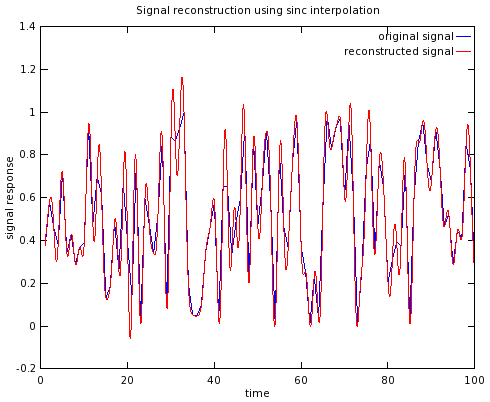
\includegraphics[scale=0.8]{background/sincreconstructed.png}
  \caption[Sinc Interpolation Approximation]{Comparison between a given random one dimensional input signal $s(t)$ and its sinc interpolation $\hat{s}(t)$. Notice that for the interpolation there were $N=100$ samples from the original signal provided.}
  \label{fig:plotsincinterpolation}  
\end{figure}

We use the sinc interpolation in order to reconstruct the DFT terms of our height field. Similarly, as discussed in section $\ref{sec:gaussianwindow}$, we reconstruct the DFT by a windowing approach. Instead of using a Gaussian window we will use the sinc interpolation. \\  

In the next chapter we talk about how to use this sinc-interpolation for rendering purposes (see section $\ref{sec:pqapproach}$). 